\documentclass{amsart}
\usepackage{graphicx}
\graphicspath{{./}}
\usepackage{hyperref}
\usepackage{csvsimple}
\usepackage{longtable}
\usepackage{epigraph}
\title{Ethnicity and Support for Political Violence and Terrorism II}
\author{Zulfikar Moinuddin Ahmed}
\date{\today}
\begin{document}
\maketitle

\section{The Result}

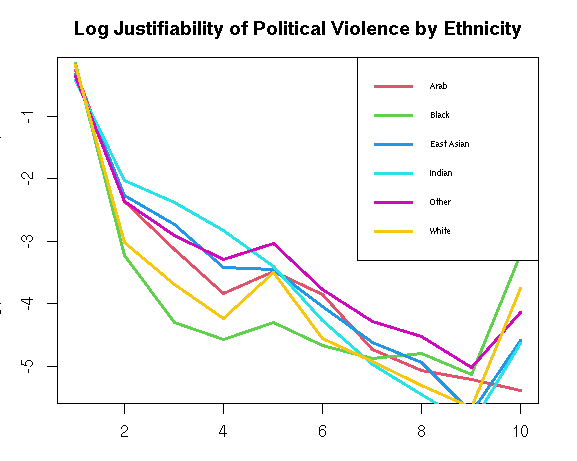
\includegraphics[scale=0.8]{ethterror.jpeg}

\section{Applications: Fix Prejudice}

Arabs have the least likely for political violence justifiability in this version, which is a major overhaul of my previous assessment.  The recommendation is to update prejudices and consider White People and Black People for the tail end more seriously, especially White people because there is a new White Supremacism effort. My previous Indian results were wrong.  Here we see tail for Indians and East Asians merge.  

\section{Major Overhaul}

I had to do some work to map World Values Survey ethnic categorisation with the six factors I used.  

\begin{verbatim}
# Create ethnicity table 
# by mapping various detailed
# country-based ethnicities to
# broader groups
library(haven)
# Problem is WVS Q290 has too many 
# gradations when we want to deal 
# with a few classes that can allow 
# us to overcome ethnic prejudices
ethnicities<-unique(as.character(as_factor(viol.eth$Q290)))

reduced_ethnicities<-function(){
  mapeth<-rep("Other",223)
  mapeth[c(1,7,15,33,38,43,65,107,154,210,214)]<-"White"
  mapeth[c(3,223,222,51,52,53,54,55,56,45,39,36,11)]<-"Black"
  mapeth[c(6,13,19,20,21,22,67,70)]<-"Indian"
  mapeth[c(4,17,48,97,98,99,100)]<-"Arab"
  mapeth[c(5,14,16,62,63,64,68,72,73,74,75,76,77,
           78,79,80,81,82,83)]<-"East Asian"
  data.frame(key=ethnicities,val=mapeth)
}

ethnicity_map<-function( v ){
  emap<-reduced_ethnicities()
  w<-sapply(as.character(as_factor(v)),
  function(x) {
  	out<-emap[which(emap$key==x),]$val;
  if(is.null(out)){
  out<-"Other"
  };
  return(out)})
  #print(head(w))
  w<-append(w,"Other")
  as.factor(unlist(w))
}

\end{verbatim}

\section{The Source of My Enormous Authority}

Already when I was in high school, in the late 1980s, there was conflict in the Middle East.  And I have seen since September 11 2001 the most atrocious transformation of American society.  Anti-Muslim propaganda, originally propagated by certain Zionist interests, had reached ungodly proportions.  Of course Arabs and Muslims had nothing whatever to do with 9/11; it was a geo-political sabotage by Israel's Mossad to trigger war plans classified by neoconservatives in America.  It was effective geostrategically, and served Israel's National Interests.  I do not worry too much about being considered 'anti-semitic' for being quite clear about the truth.  

My convictions were always that the mischaracterisation of Arabs in America was inaccurate.  So the above result, which shows with substantial amount of high quality data, that Whites are more likely to hold extreme views about justifiability of political violence compared to Arabs, is not surprising at all to me, and I am very pleased to discover this in a serious data set.  The characterisation of Arab Muslims are having more propensity for political violence than other people is a conscious malicious war propaganda attempt that I think originates with the Likud elements of Israel, especially the coterie of Isser Harel and other old schoolers.  America fell for this war propaganda.  I am nixing it now.  This is deep truth at the hands of someone who has quite good intuition of how people are like.


\section{Examination of Data Validity}

In this note I am making a very strong claim about the world we live in.  I am claiming that White people are significantly more likely to hold extreme views about justifiability of political violence, i.e. terrorism, than Arabs.  I am obviously interested in being accurate with respect to Nature about this claim.  I am well aware that this claim flies against the face of war propaganda of several decades in America and therefore it is worthwhile checking carefully whether this claim, this {\em scientific discovery} has merit.  I did not know what my analysis would show because global level survey data are still not fully understood.  

So let us first of all check sample sizes; we are making claims based on these.

% latex table generated in R 4.0.3 by xtable 1.8-4 package
% Sun May  2 02:37:09 2021
\begin{table}[ht]
\centering
\begin{tabular}{rlr}
  \hline
 & eth & N \\ 
  \hline
Arab & Arab & 3513 \\ 
  Black & Black & 2898 \\ 
  East Asian & East Asian & 9064 \\ 
  Indian & Indian & 1874 \\ 
  Other & Other & 31784 \\ 
  White & White & 11165 \\ 
   \hline
\end{tabular}
\end{table}

We want to keep focus on Arabs and Whites because this is very serious politically and we want Washington and London and Western Capitals have very clear understanding of these data, because the mischaracterization of Arabs as particularly prone to terrorism is egregiously inaccurate and wrong.  $N_{Arabs}=3513$ here and $N_{Whites}=11165$.  These are both large samples to produce extremely strong inferences.  We will make the inference that Whites are strongly significantly likely to hold extreme terrorist support views than Arabs.  We will ignore the other ethnicities until we are extremely clear about this clear strong inference.


\section{Probability of Anti-Terrorism Views}

We define anti-terrorism view as the views that find political violece unjustifiable.  We consider 1--5 as reasonable anti-terrorism view.

% latex table generated in R 4.0.3 by xtable 1.8-4 package
% Sun May  2 02:52:54 2021
\begin{table}[ht]
\centering
\begin{tabular}{rlr}
  \hline
 & eth & nonviol \\ 
  \hline
Arab & Arab & 0.9536 \\ 
  Black & Black & 0.9289 \\ 
  East Asian & East Asian & 0.9521 \\ 
  Indian & Indian & 0.9626 \\ 
  Other & Other & 0.9300 \\ 
  White & White & 0.9506 \\ 
   \hline
\end{tabular}
\end{table}

Note that more than 90\% of all ethnicities are anti-terrorism.  This is important, because our claim will not be that Whites are pro-terrorism.  

{\em No ethnicity is pro-terrorism}

\section{Focus on right tail to seek significance in extremism difference}

We look at 9--10 on agreement with political violence is justified.  Let is refer to these as $\mu_{White}, \mu_{Arab}$ etc.  Then let $\sigma$ denote the standard deviation of the percentages.  We have:

\[
\frac{\mu_{Whites} - \mu_{Arabs}}{\sigma} = 1.248
\]

Fine White Terrorism agreement is not $2\sigma$ more than Arabs, but $1.248\sigma$.  That's not small.  That is significant  too if we're looking at levels 9--10.

Now let's look at just level 10, extreme comfort with justifiability with political violence.  Let's keep the same notation, this time only level 10.

\[
\frac{\mu_{Whites} - \mu_{Arabs}}{\sigma} = 1.46
\]
It's more significant here as well.

\section{Conclusion:White Agreement with Extreme Terrorist Violence is higher than Arabs}

This is a very serious conclusion, and one that needs to be considered seriously in all Western capitals.  We cannot have a world that runs reasonably if senior policy makers make decisions based on bullshit.


\end{document}